\documentclass[%
 reprint,
%superscriptaddress,
%groupedaddress,
%unsortedaddress,
%runinaddress,
%frontmatterverbose, 
%preprint,
%preprintnumbers,
%nofootinbib,
%nobibnotes,
%bibnotes,
 amsmath,amssymb,
 aps,
%pra,
%prb,
%rmp,
%prstab,
%prstper,
%floatfix,
]{revtex4-2}

\usepackage{graphicx}% Include figure files
\usepackage{dcolumn}% Align table columns on decimal point
\usepackage{bm}% bold math
\usepackage{physics}
\usepackage{cancel}
\usepackage{float}
\usepackage{blindtext}
%\usepackage{hyperref}% add hypertext capabilities
%\usepackage[mathlines]{lineno}% Enable numbering of text and display math
%\linenumbers\relax % Commence numbering lines

%\usepackage[showframe,%Uncomment any one of the following lines to test 
%%scale=0.7, marginratio={1:1, 2:3}, ignoreall,% default settings
%%text={7in,10in},centering,
%%margin=1.5in,
%%total={6.5in,8.75in}, top=1.2in, left=0.9in, includefoot,
%%height=10in,a5paper,hmargin={3cm,0.8in},
%]{geometry}

\begin{document}

\preprint{APS/123-QED}

\title{Survey of Computational Methods for Plasmas}% Force line breaks with \\

\author{Evan Bluhm}
%  \altaffiliation[Also at ]{Physics Department, XYZ University.}%Lines break automatically or can be forced with \\
% \author{Second Author}%
%  \email{Second.Author@institution.edu}
% \affiliation{%
%  Authors' institution and/or address\\
%  This line break forced with \textbackslash\textbackslash
% }%


\date{June 04, 2021}% It is always \today, today,
             %  but any date may be explicitly specified
\begin{abstract}

\blindtext
% % \begin{description}
% % \item[Usage]
% % Secondary publications and information retrieval purposes.
% % \item[Structure]
% % You may use the \texttt{description} environment to structure your abstract;
% % use the optional argument of the \verb+\item+ command to give the category of each item. 
% % \end{description}
\end{abstract}

%\keywords{Suggested keywords}%Use showkeys class option if keyword
                              %display desired
\maketitle

%\tableofcontents

\section{Introduction}


\blinddocument
% \begin{figure}[H]
% 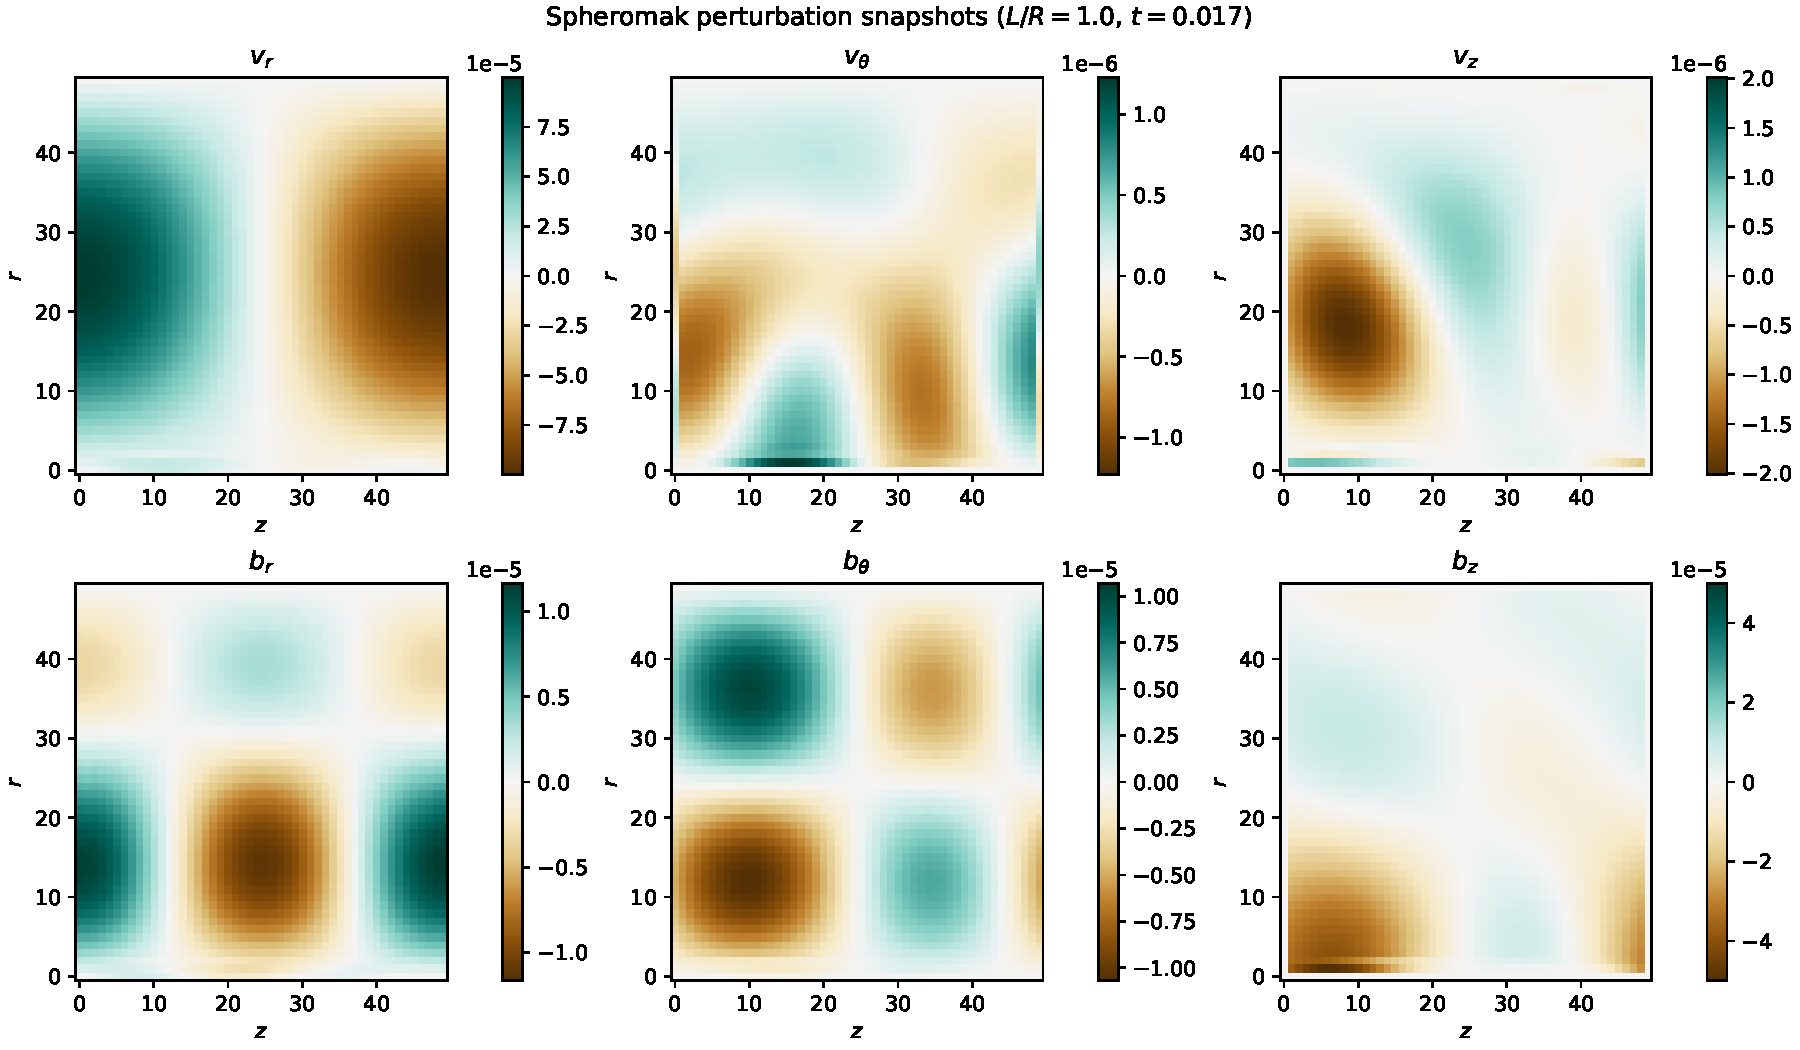
\includegraphics[width=0.9\linewidth]{proj2-3/spheromak_snapshot_1.pdf}
% 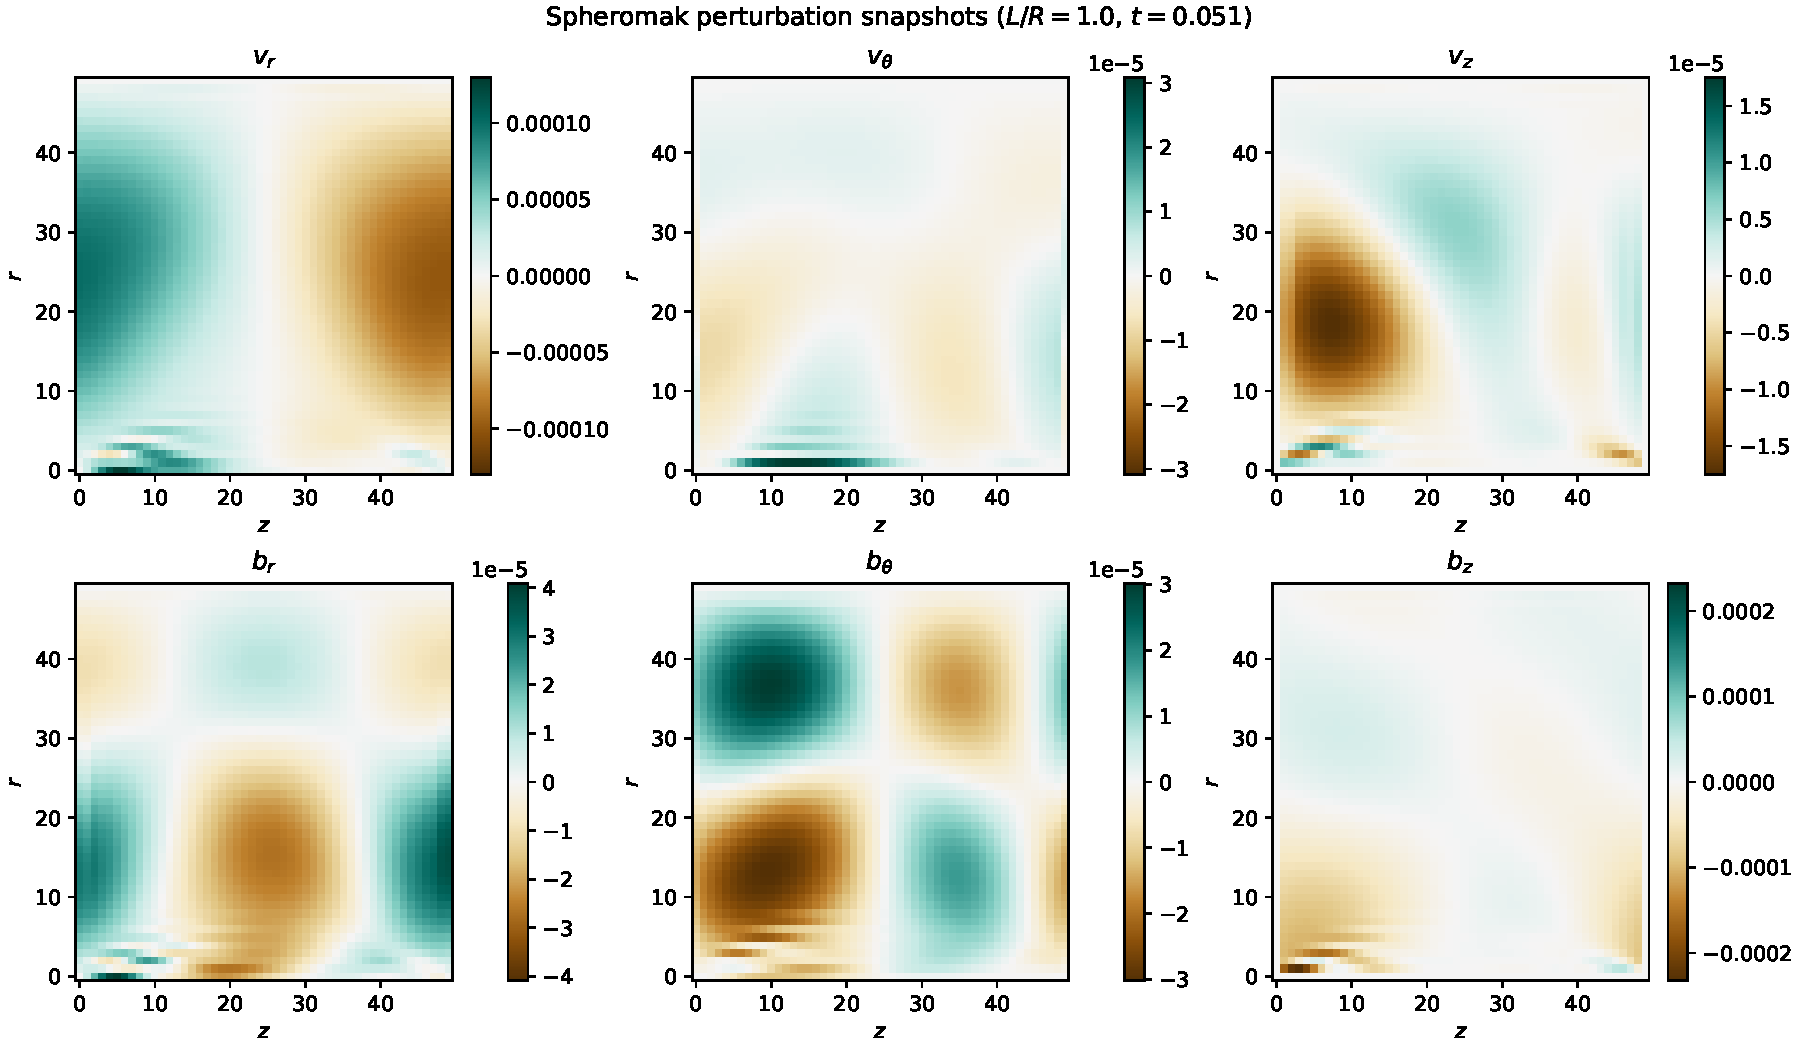
\includegraphics[width=0.9\linewidth]{proj2-3/spheromak_snapshot_3.pdf}
% 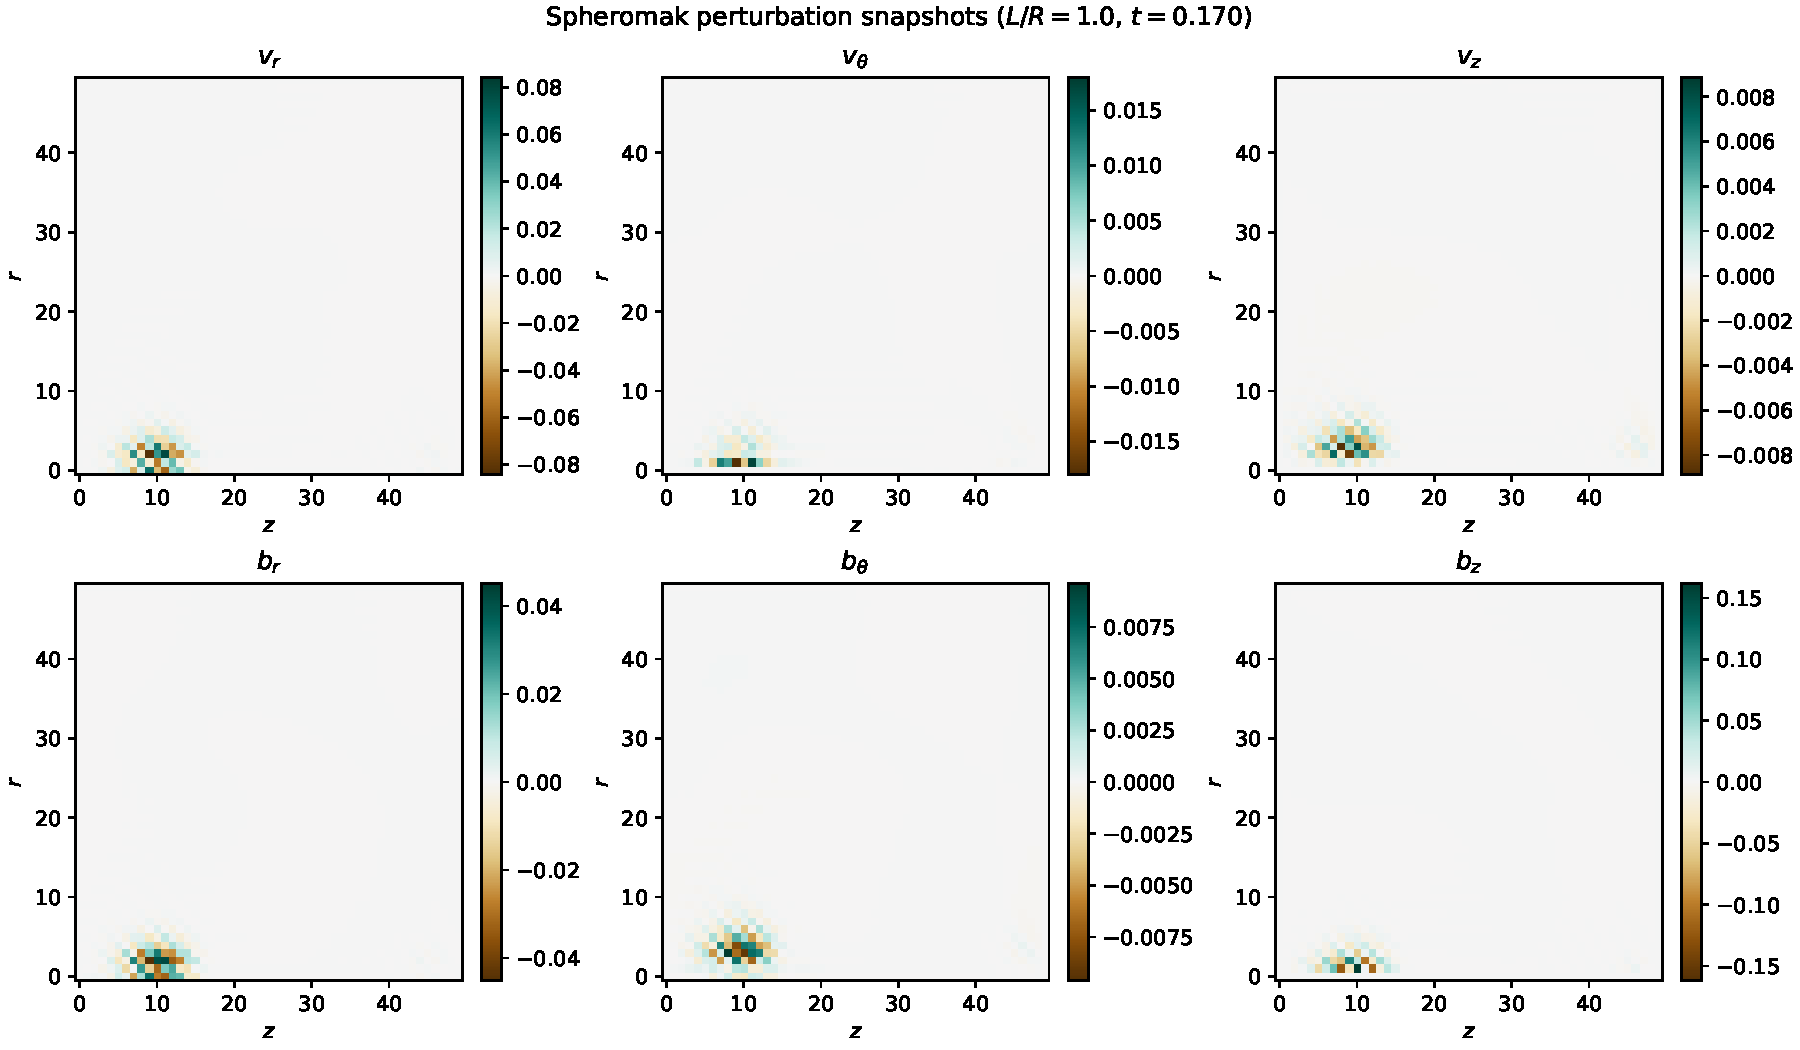
\includegraphics[width=0.9\linewidth]{proj2-3/spheromak_snapshot_10.pdf}
% \caption{\label{fig:spheromak-instability-snapshots}Snapshots of the perturbation solution in time, for the initial conditions shown in Figure \ref{fig:spheromak-initial-conditions}. The model parameters are $M_r=50$, $M_z=50$, $\delta =0.0001$, $\Delta t=0.001$, and $L/R=1.0$. These snapshots show the growth of a numerical instability in time near the axis of symmetry. Stationary errors begin to grow, until they dominate the solution by $t=0.1$.}
% \end{figure}



\nocite{*}

\bibliography{summary}% Produces the bibliography via BibTeX.


\onecolumngrid

\pagebreak

\appendix

\end{document}
